\pattern{Facade}
\begin{summary}
    The goal of a {\bf Facade} is to create an object that provides a simplified,
    unified interface to a more complex, larger body of code such as the
    various interfaces of a subsystem. 
\end{summary}

\comparison{\begin{itemize}
        \item Low Coupling: Clients are decoupled from a subsystem. Avoid tight
            coupling between a client and it’s subsystem by introducing an
            independent facade interface
        \item Readability: Simplify complex code blocks and provide convenient
            methods. Wrap several code blocks to a more elegant set of APIs.
        \item Maintainability: Facade provides a single point of entry to a
            subsystem, improving usability and simplicity.
\end{itemize}

}{\begin{itemize}
        \item Efficiency: Adds a layer to the code stack, which may affect
            performance.
        \item Readability: Developers still need to know implementation
            details, and the pattern will increase the size of the code base.
        \item Evolvability/Adaptability: if the Facade is the only access point
            for the subsystem, it will limit the features and flexibility that
            ``power users'' may need.
\end{itemize}
}% END comparison

\begin{nfps}
\item[Complexity] The pattern allows the client to work through this singular
interface to existing subsystem components. 
\item[Evolvability] Working through a Facade minimizes dependencies for the
client, making it easier to implement, change, and use.
\end{nfps}

\subsubsection{Example}
Facade is an extremely versatile pattern, able to be applied to various
situations. This can include:\begin{itemize}
\item Database access
\item Network communication
\item Any code libraries
\item Input/output interfaces
\end{itemize}

Real life example is the customer service department at any company. The
company handles many things such as sales, returns, order inquiries and
shipping. It would be very annoying if you had to access any of these
departments through different means, however the use of a customer service
department acts as a facade and simplifies the process.

\begin{center}
    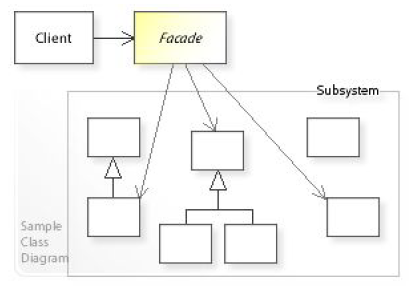
\includegraphics[width=0.8\textwidth]{./facade}
\end{center}
